\documentclass[]{article}
\usepackage[paperheight=18cm,paperwidth=18cm]{geometry}
\usepackage{tikz}
\usepackage{pgfplots}
\usepackage{mathrsfs, amssymb, amsfonts}
\pgfplotsset{compat=1.11, width=14cm}
\usetikzlibrary{calc}
\pagecolor{gray}

\tikzset{axis line style/.style={thin, gray, -stealth}}


%opening
\title{Represtation of the fonctions Cos and Sin}

\begin{document}

\thispagestyle{empty}
\begin{center}
		\begin{center}
		 \huge \color{white} \textbf{Represtation of the fonctions Cos and Sin}	
	
	\end{center}

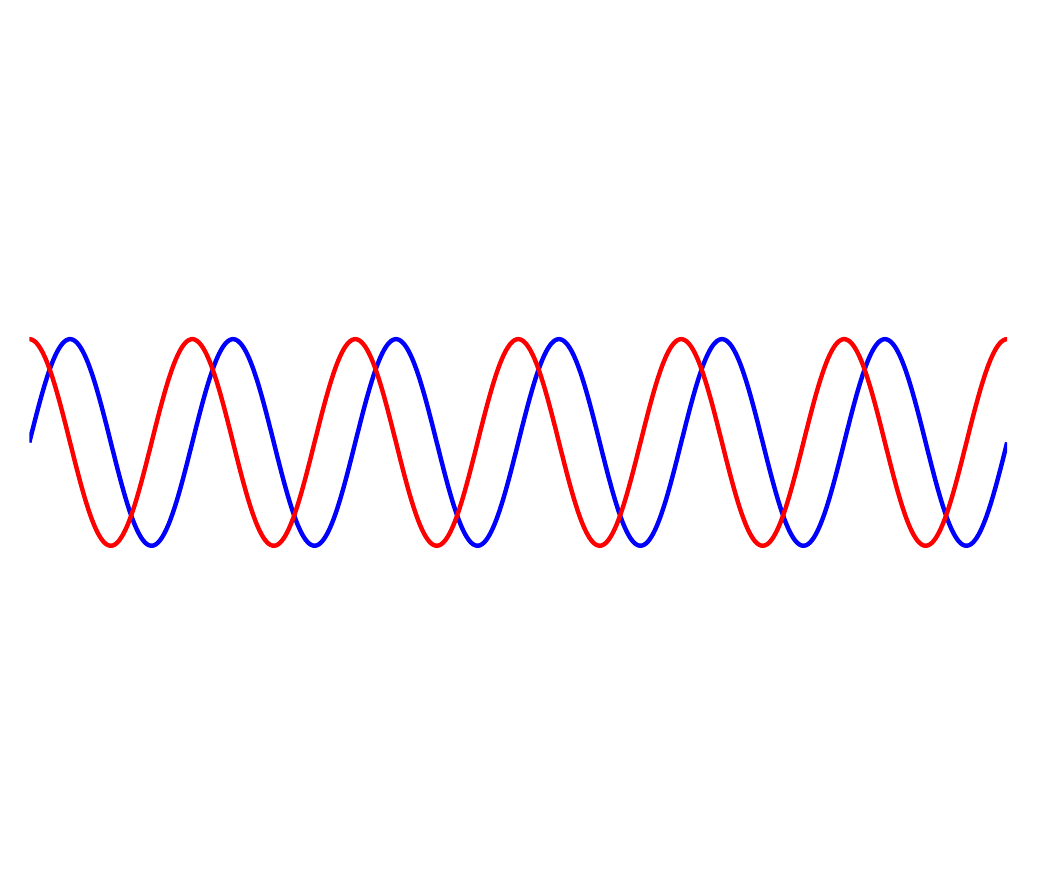
\begin{tikzpicture}
	\begin{axis}[
		axis line style={->, white, very thick},
		xtick=\empty, ytick={-1,1},,yticklabel={$\color{white}\pgfmathprintnumber{\tick}$}, tick style={white, ultra thick},
		xlabel= \color{white}$x$,
		ylabel= \color{white}{$y$},
		domain=-6*pi:6*pi,
	    samples=1000,
		axis lines=middle, ymin=-4, ymax=4
		]
		
		\addplot[blue, ultra thick] {sin(deg(x))};
		\addplot[red, ultra thick]{cos(deg(x))};
		
			
	
	\end{axis}

\end{tikzpicture}
\color{white} \small
\#AEK
\end{center}
\end{document}
